% ==============================================================================
\section{Módulo de alertas}
\label{sec:dev_alertas}
% ==============================================================================

\subsection{Descripción}

El módulo de alertas es la capa de seguridad del sistema y corresponde al Algoritmo 7
de TT1. La navegación solo trabaja cuando hay una ruta activa, pero las alertas están
encendidas todo el tiempo, así que una persona puede usar los lentes sin pedir ningún
destino y aun así enterarse de lo que tiene enfrente. El módulo atiende RF-12, RF-20,
RNF-01, RNF-09 y RNF-12.

En cada ciclo, \texttt{alertas.py} lee el cuadro de navegación y regresa la lista de
alertas nuevas, cada una con su prioridad, junto con una bandera que indica si hay que
recalcular la ruta. También se encarga del sonido. Para esa parte se integró el módulo
de pitidos que desarrolló el equipo (\texttt{VozYPLN/alertas.py}), y gracias a él las
alertas no se confunden con las indicaciones de navegación. Una precaución es solo un
pitido estéreo, mientras que una alerta crítica es un pitido seguido de una frase corta
que interrumpe cualquier otra cosa que el sistema esté diciendo.

\subsection{Reglas de alerta}

La Tabla~\ref{tab:alertas_reglas} reúne las reglas. Los umbrales del frente (0.80~m
para la alerta crítica y 1.50~m para la precaución) son los definidos en TT1. En los
costados los umbrales son menores, porque caminar a 60~cm de una pared es lo más normal
en un pasillo y no amerita una alerta crítica. La excepción son las detecciones de
riesgo alto, que usan los umbrales del frente en cualquier sector.

\begin{longtable}{|p{3.4cm}|p{3.6cm}|p{3.2cm}|p{4.3cm}|}
\caption{Reglas del módulo de alertas}
\label{tab:alertas_reglas} \\
\hline
\textbf{Situación} & \textbf{Crítica} & \textbf{Precaución} & \textbf{Ejemplo de
frase} \\
\hline
\endfirsthead
\hline
\textbf{Situación} & \textbf{Crítica} & \textbf{Precaución} & \textbf{Ejemplo de
frase} \\
\hline
\endhead
Obstáculo al frente (mapa o visión) & $< 0.80$~m & $< 1.50$~m & ``Atención:
obstáculo a 80 centímetros al frente. Deténgase.'' \\
\hline
Obstáculo a un costado & $< 0.45$~m & $< 0.80$~m & ``Precaución: obstáculo cerca a
la izquierda.'' \\
\hline
Persona u objeto en movimiento (hasta 2~m) & $< 1.0$~m & de 1.0 a 2.0~m & ``Alto. Se
acerca una persona al frente, muy cerca.'' \\
\hline
Hoyo, agua o escalera al frente (hasta 2.5~m) & $< 1.3$~m & de 1.3 a 2.5~m &
``Atención: un hoyo adelante, a unos 2 pasos.'' \\
\hline
Eco ultrasónico que ninguna detección confirmada explica & $< 0.80$~m & de 0.80 a
1.50~m & ``Atención: pared al frente a 60 centímetros. Deténgase.'' \\
\hline
Detección contradicha por el ultrasonido (al frente) & --- & $< 1.5$~m & ``Posible
silla al frente (solo cámara).'' \\
\hline
Lectura directa de un sensor de proximidad & $< 1.0$~m & de 1.0 a 1.5~m & Pitido
inmediato en la dirección del eco. \\
\hline
\end{longtable}

Si hay una persona en movimiento en un sector, su aviso reemplaza al aviso genérico de
obstáculo de ese sector, para no decir dos cosas sobre lo mismo. Los peligros de piso se
describen en pasos, contando 0.7~m por paso, porque es una medida que el usuario puede
ir contando mientras camina. Las distancias del texto se redondean a múltiplos de
10~cm para que el ruido de la estimación no cambie la frase en cada ciclo, y los objetos
se nombran en español con el mismo diccionario que usa la interacción
(Sección~\ref{sec:dev_interaccion}), de modo que el detector dice \emph{chair} pero el
usuario escucha ``silla''.

Los dos ultrasónicos frontales agregan tres reglas más. Un eco cercano que ninguna
detección confirmada por la cámara explica se avisa como pared u obstáculo; así se
cubren los vidrios, las mamparas y las paredes lisas, que la visión no reconoce. Si los
dos sensores miden casi lo mismo, se trata de una superficie de frente y el aviso dice
``pared''; si solo uno la detecta, el objeto está cargado hacia ese lado. Este aviso
reemplaza al genérico de esa dirección, porque el ultrasonido mide con más precisión que
el mapa. En cambio, una detección visual que el ultrasonido contradice, porque el haz
debería alcanzarla y no hay eco a esa distancia, ya no dispara una alerta crítica con la
distancia de la cámara. Se avisa solo como precaución, con la frase ``posible\dots{}
(solo cámara)'', siguiendo la idea de RNF-09 de avisar sin alarmar de más.

La tercera regla es de rapidez. Las lecturas no esperan al ciclo de visión; la función
\texttt{conectarUltrasonido} revisa cada lectura nueva y, si hay un eco a menos de 1.5~m,
suena un pitido de inmediato en su dirección. Antes se descartan los ecos del piso con
el cabeceo de la IMU, y la lectura mínima del sensor, 20~cm, se interpreta como ``20~cm
o menos'' y produce un pitido crítico, porque es la situación más peligrosa. La alerta
correspondiente llega al navegador en el siguiente ciclo. Como los dos sensores se
disparan por turnos y cada medición toma 100~ms, cada uno se actualiza unas cinco veces
por segundo.

\subsection{Dosificación y recálculo}

Si una alerta se repitiera en cada ciclo, el usuario recibiría diez avisos por segundo.
Para evitarlo, cada alerta tiene un tiempo de espera antes de volver a sonar, de 2.5~s
para las críticas y de 8~s para las precauciones. El tiempo se cuenta por prioridad,
por dirección (frente, izquierda o derecha) y por tipo de aviso (obstáculo, persona en
movimiento o peligro de piso), de modo que una precaución por algo a la izquierda no
silencia una precaución por algo al frente.

Esta forma de agrupar se definió después de dos intentos. Primero, el tiempo de espera
se aplicaba al texto exacto de la frase, pero como la distancia cambia de un ciclo a
otro, cada frase resultaba ``nueva'' y no se filtraba nada. Después se agrupó por el
inicio del texto, y en las pruebas del escenario que se describe más adelante una
precaución lateral llegó a silenciar durante 8~s la precaución frontal de una pared.

Cualquier alerta crítica activa la bandera de recálculo. El navegador la recibe y decide
en ese mismo ciclo, sin esperar su intervalo de un segundo, y el planificador de ruta
recalcula de inmediato. Las alertas se pueden apagar y encender con la tecla \texttt{x}
en la computadora portátil y con un doble clic del botón físico en el prototipo.

\subsection{Pitidos estéreo}

El módulo de pitidos del equipo genera los tonos por software y los reproduce en un hilo
propio, de modo que suenan aunque el programa principal esté escuchando o hablando. La
dirección se codifica con el balance entre canales; un obstáculo a la izquierda suena
fuerte en el oído izquierdo y bajito en el derecho, y uno al frente suena igual en ambos.
El nivel se codifica con el patrón (Figura~\ref{fig:alertas_pitidos}). La alerta
crítica son cuatro tonos cortos que alternan entre 2100 y 1500~Hz, y la precaución, dos
tonos de 1200~Hz más largos. Mientras suena un pitido la cola de voz espera, y si llega
una alerta crítica mientras el sistema habla, la frase en curso se corta.

\begin{figure}[H]
    \centering
    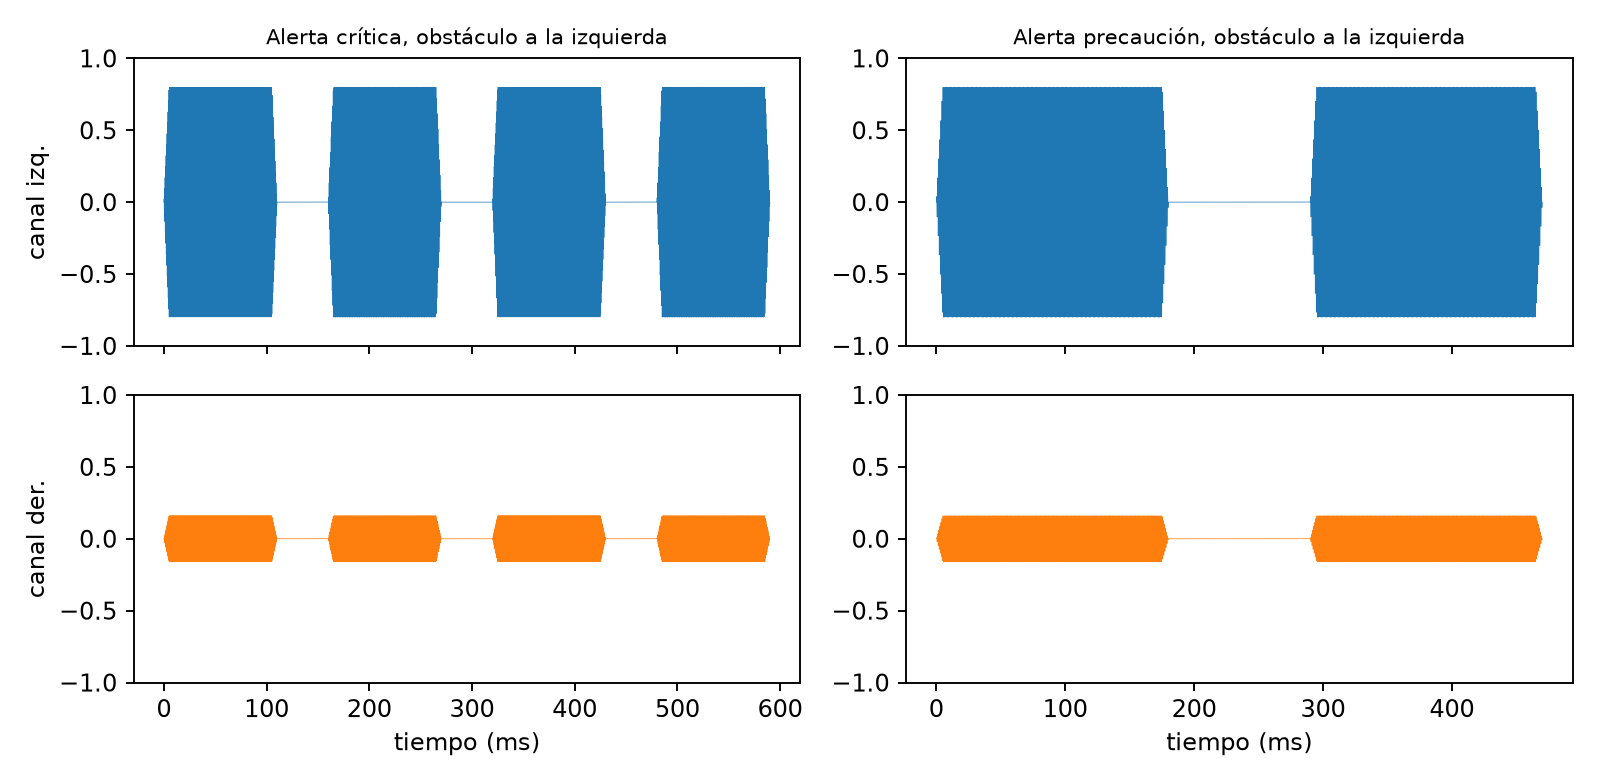
\includegraphics[width=0.88\textwidth]{Capturas_TT2/nav/alertas_pitidos.png}
    \caption{Forma de onda de los pitidos para un obstáculo a la izquierda, con la alerta
    crítica a la izquierda y la precaución a la derecha. El canal derecho suena al
    20\,\% del volumen del izquierdo.}
    \label{fig:alertas_pitidos}
\end{figure}

El módulo del equipo trae también su propia lógica para decidir el nivel; por ejemplo,
un vehículo a menos de 5~m es crítico, y si un sensor y la cámara reportan lo mismo en la
misma dirección casi al mismo tiempo, la alerta sube un nivel. En el sistema integrado
esa lógica no se usa, porque el nivel lo decide \texttt{alertas.py} con las reglas de la
Tabla~\ref{tab:alertas_reglas} y el módulo del equipo solo se encarga de sonar.

\subsection{Resultados}

\textbf{Pruebas con el prototipo.} \TODO{escenarios probados con el prototipo (por
ejemplo, acercarse a una pared, a una puerta de vidrio y a una persona), alertas
esperadas contra alertas emitidas, falsas alarmas y si los participantes distinguieron
la dirección de los pitidos}.

\textbf{Escenario simulado.} Para revisar el comportamiento de las reglas se preparó un
escenario en el cuarto simulado, en el que el usuario camina en línea recta hacia la
pared del fondo mientras una persona le cruza por delante. La
Figura~\ref{fig:alertas_escenario} muestra la distancia libre al frente según el mapa,
la distancia estimada a la persona y las alertas que emitió el módulo, 14 en total en
17~s.

\begin{figure}[H]
    \centering
    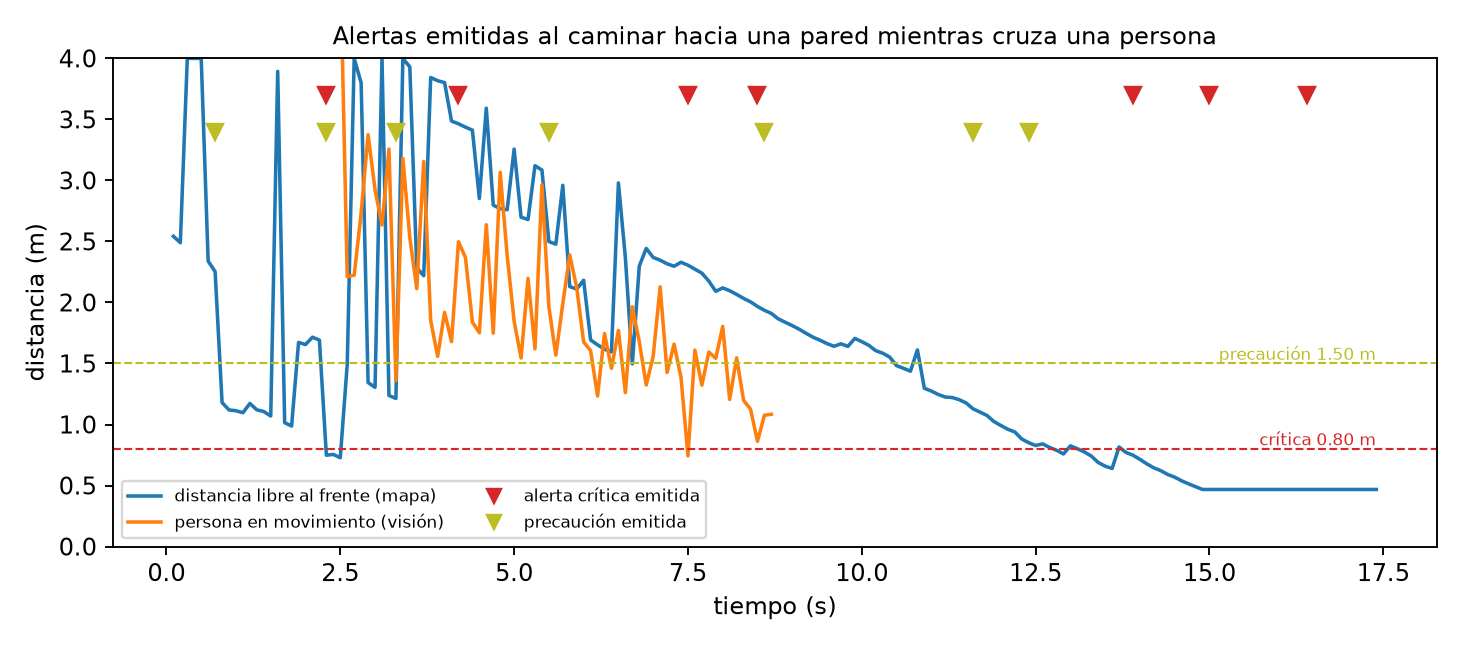
\includegraphics[width=\textwidth]{Capturas_TT2/nav/alertas_escenario.png}
    \caption{Alertas emitidas en el escenario de prueba. Los triángulos marcan cada alerta
    crítica (rojo) y cada precaución (verde).}
    \label{fig:alertas_escenario}
\end{figure}

La persona se avisó como se esperaba. A los 3.3~s, ya a menos de 2~m, sonó ``Precaución:
una persona en movimiento al frente'', y a los 7.5~s, a menos de 1~m, la alerta crítica
``Alto. Se acerca una persona al frente, muy cerca''. Al seguir su camino, la persona
quedó del lado derecho del usuario y el aviso cambió de dirección (8.5~s). Después el
ultrasonido detectó la pared, primero con precauciones a los 11.6 y 12.4~s y luego con
alertas críticas a los 13.9, 15.0 y 16.4~s, la última a 51~cm, porque el usuario siguió
avanzando. Entre los 12.6 y los 13.9~s el mapa ya marcaba menos de 0.80~m, pero el eco,
que mide la distancia real, todavía estaba por encima del umbral; como el aviso del
ultrasonido reemplaza al del mapa en esa dirección, la alerta crítica esperó a que el
eco bajara.

La prueba dejó ver dos efectos que conviene tener presentes. El primero es que el
cálculo estéreo del lado oscila cuando el usuario se acerca a una pared con un ligero
ángulo, de modo que la misma pared se reporta unas veces ``al frente'' y otras
``adelante a la derecha''. Como la dosificación cuenta cada dirección por separado, eso
produjo cinco avisos por la misma pared en menos de cinco segundos. \TODO{agrupar los
avisos del ultrasonido en una sola dirección frontal cuando ambos sensores ven la misma
superficie}. El segundo es que al inicio sonaron alertas por la mesa y el sillón que
quedaban a los lados, algunas con una distancia menor a la real. El escenario parte de un
mapa construido en un recorrido previo y la pose inicial se fijó a mano, así que hay un
desajuste entre la pose y el mapa; en una corrida de prueba se comprobó que, con la pose
desplazada 0.4~m, una pared ya registrada aparecía a 40~cm en un costado donde no había
nada.

En cuanto al tiempo, evaluar las reglas toma en promedio 0.007~ms por ciclo, así que lo
que tarda una alerta en sonar desde que el obstáculo aparece en la imagen depende de la
visión, unos 160~ms por cuadro en la computadora portátil. En el prototipo esa latencia
es de \TODO{latencia de alerta medida en la Raspberry Pi}, contra los 2~s que permite
RNF-01. El módulo tiene 26 pruebas automatizadas junto con el planificador de ruta.

\subsection{Limitaciones}

Las alertas heredan los errores de la percepción. Un tapete detectado como hoyo provoca
una alerta falsa, y un obstáculo que la cámara no reconoce y que no devuelve eco, como
un objeto bajo y muy cercano, no provoca ninguna. Tampoco hay alertas para lo que queda
detrás o muy a los costados del usuario, porque ni la cámara ni los ultrasónicos cubren
esas zonas.
